\documentclass{article}
\usepackage[utf8]{inputenc}
\usepackage[margin=1in]{geometry}
\usepackage{mathptmx}
\usepackage{mathtools}
\usepackage{amsmath}
\usepackage{subcaption}
\setlength{\parindent}{0em}
\setlength{\parskip}{0.5em}


\title{Assignment 3 - CTA200}
\author{Rishik Adhikari}
\date{May 11, 2023}

\usepackage{natbib}
\usepackage{graphicx}

\begin{document}

\maketitle

\section*{Question 1}

In, this question, we are dealing with complex numbers, writing a modular file to import a function from, and plotting using various methods. Initially, we are given some initial conditions, such as for each points in the complex plane: $c = x + yi$, we start with $z_0 = 0$ where $-2 < x < 2$ and $-2 < y < 2$. We iterate the $z_i$ using the equation: $z_{i + 1} = z_i^2 + c$. We can choose how many times we would like to iterate the $z_i$ and based on that define if a point in the complex plane $c$ is bounded or diverges to $\infty$. The boundary condition is given by: $|z|^2 = Re(z)^2 + Im(z)^2$.

For the Plotting Part: We are required to plot in a complex plane, bounded and divergent complex points. One normally, and another similar plot where the divergent points get color in a gradient like format, using an iteration tracker.  

The solution follows like this: 
Make 2 numpy arrays of size n to create the complex number c. Then, use a nested loop to loop over them to cover all the points. After that, set $z_0 = 0 $. You are given or you pick by yourself the number of iterations to iterate for each complex point c. $z_i$ is iterated accordingly and at the end of the N number of iterations, the boundary condition is checked and the complex point is classified as bounded or divergent and appended into the co responding list for future plotting. 
In this entire process, we can also keep track of the iterator for the second plot for divergent points, which will reduce the run-time of the program requiring us to run the entire process once instead of twice. 
\\
For Plotting Section, Please refer to the code on GitHub.

\begin{figure}[!htb]
    \centering
    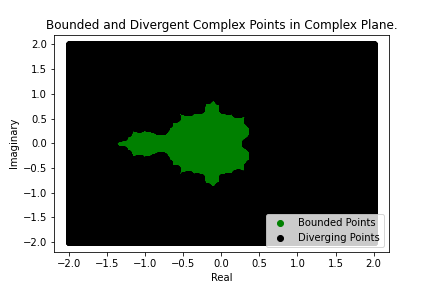
\includegraphics[scale=0.7]{q1_1.png}
    \caption{ First Plot among two of the points in the complex planes. Colour is based on whether the points are bounded or diverge to $\infty$.}
    \label{fig:q1_1.png}
\end{figure}

\begin{figure}[!htb]
    \centering
    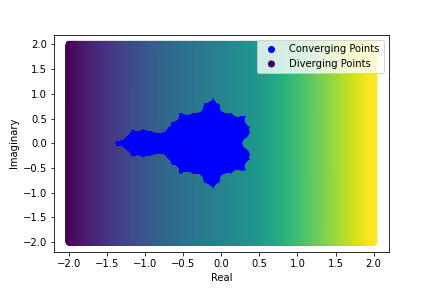
\includegraphics[scale=0.9]{q1_2.png}
    \caption{ Second Plot among two of the points in the complex planes. Colour is based on whether the points are bounded or diverge to $\infty$. Divergent Points have a gradient colour or colour scale. }
    \label{fig:q1_2.png}
\end{figure}
\newpage
One Quick thing we can notice from the plot is that, the points that are bounded are closer to the origin. Beside, that the outcome is a really beautiful looking object created mathematically using a computer program. 

This Question helps to practice, plotting, getting comfortable with complex numbers and complex planes in python, writing our own module to modularize the code for distribution or any other purpose.  

\section*{Question 2}

Question 2 is about replicating a numerical computation done by the researcher, Edward Lorenz, in his research paper titled: "Deterministic Nonperiodic Flow". This paper demonstrates that deterministic physical systems could exhibit unpredictable behavior. 

We are given some initial values w = [$x_0, y_0, z_0$]. Along with some constants $\sigma, r$ and $b$. 
This Question is further divided into subsection, so I will summarize them as one. \\\\

The steps for solutions are as follows: \\\\
1) Create A function f(initValues, time, args=(sigma,r,b)), to pass into the odeint solver from scipy library. \\\\
2) Initialize all the given initial values such as w, sigma, r and b. And also create a time array using numpy with timeDelta = 0.01. [You can use: t = numpy.arange(0,60,0.01)]. Also, create an array N where N = t/timeDelta. the next plot uses N instead of t for plotting.\\\\
3) Solve the differential equation using the odeint function from scipy library. [Please refer to the documentation for how to use it.]\\\\
4) Reproduce the Figure 1 from the Lorenz Paper. User Matplotlib subplots, it will easily help to build the required plot. Make sure to have separate plt.xlim or axs[i].set\_xlim for the three different graphs.\\\\ 
5) Reproduce the Figure 2 from the Lorenz Paper. Again, utilize the Matplotlib subplots. You do not need to solve the ODE again and again, the results from previous section should be good.\\\\
6) Now change the initially given values w with w'. w' is also given, but a list addition needs to be performed which cannot be directly done in python. However, convert both lists to numpy arrays using np.array(listName) and perform the normal addition w' = w + givenList. Again convert the numpy arrary, w' to list using list(w'). this is more easier than using a for loop or any other looping techniques including but not limited to list comprehension using lambdas.  \\\\
7) Solve the ODE again using the new w' values. Everything else is same.\\\\
8) Calculate the distance between the two different solutions. Using the distance Foromula: $\sqrt{(x_2 - x_1)^2 + (y_2-y_1)^2 + (z_2-z_1)^2}$. Please Refer to GitHub  Code for working Code.\\\\
9) Plot a distance vs time graph using a semi-log scale. Distance -> log scale, Time -> linear Scale. You can use plt.yscale("log") to the set the scale of y-axis to log-scale. \\\\
10) Observe and Report.\\\\

All The Plots of Question 2 Are Embedded Below. 

\begin{figure}[!htb]
  \centering
  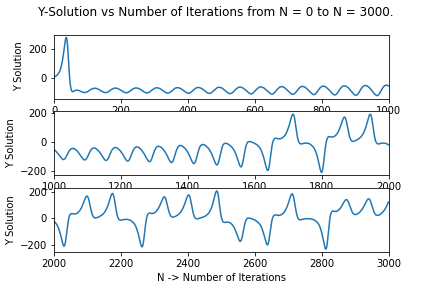
\includegraphics[width=1\linewidth]{q2_1.png}
  \caption{}
  \label{fig:q2_1.png}
\end{figure}


\begin{figure}[!htb]
  \centering
  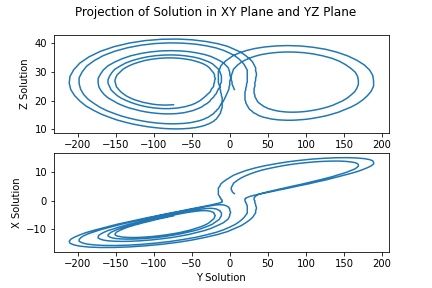
\includegraphics[width=1\linewidth]{q2_2.png}
  \caption{}
  \label{fig:q2_2.png}
\end{figure}

\begin{figure}[!htb]
  \centering
  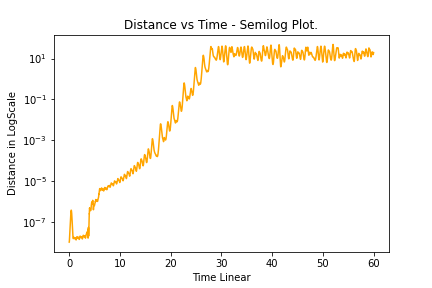
\includegraphics[width=1\linewidth]{q2_3.png}
  \caption{In this Last, Plot we can see that the log scale shows a closer to linear Line Pattern, which in linear scale would refer to exponential growth. So, from here we can see that even a small change in the initial value can impact the system a lot. }
  \label{fig:q2_3.png}
\end{figure}




\end{document}